\documentclass[oneside,a4paper]{memoir}

\usepackage{microtype}
\usepackage{graphicx}
\usepackage{subcaption}
\usepackage{textcomp}

\usepackage[sc]{mathpazo}
\linespread{1.05}

\usepackage{menukeys}

\usepackage{minted}
\setminted{frame=lines}

\usepackage{hyperref}
\usepackage{xcolor}
\hypersetup{
    colorlinks,
    linkcolor={red!80!black},
    citecolor={red!50!black},
    urlcolor={blue!50!black},
    filecolor={blue!50!black}
}

\usepackage{tikz}
\usetikzlibrary{arrows.meta}

\semiisopage
\checkandfixthelayout

\chapterstyle{bianchi}
% Changing the fonts a bit
\renewcommand*{\chapnamefont}{\normalfont\huge\itshape}
\renewcommand*{\chaptitlefont}{\normalfont\Huge}
\renewcommand*{\printchaptertitle}[1]{%
  \hrule\vskip\onelineskip \centering \chaptitlefont #1\par}

% Adapted from https://tex.stackexchange.com/a/315324/155372
\newcommand{\grid}[2][blue!75]{
\fill[#1]
  \foreach \row [count=\y] in {#2} {
    \foreach \cell [count=\x] in \row {
      \ifnum\cell=1 %
        (\x-1, -\y+1) rectangle ++(1, -1)
      \fi
      \pgfextra{%
        \global\let\maxx\x
        \global\let\maxy\y
      }%
    }
  }
;
\draw[thin] (0, 0) grid[step=1] (\maxx, -\maxy);
}

\newcommand\hreftt[2]{\href{#1}{\texttt{#2}}}

\begin{document}

\title{Cabasa: User Manual}
\preauthor{}\postauthor{}\author{} % removes extra space when no author is given
\maketitle

\tableofcontents

\chapter{Introduction}

Cabasa is an application for the simulation of arbitrary 2D cellular automata.

\section{What is a Cellular Automaton?}
\label{sec:whatisca}

\textbf{Note:} You can skip this section if you already know about cellular automata.

\vspace{2ex}

A \emph{cellular automaton} (abbreviated from now on as CA/CAs) is a type of mathematical simulation which operates on a set of \emph{cells}.
The cells are arranged in some sort of lattice (typically a 1D line or a 2D grid).
Each cell has an associated \emph{state}, which is one value drawn from a predefined set of values.

On each step of the simulation, a fixed set of rules is applied.
Each step is referred to as a \emph{generation}.
A pattern starts at generation 0, and each time the rules are applied the generation is increased by one.

To illustrate this, consider the well-known CA known as \emph{Conway's Game of Life} (or \emph{Life} for short).
This CA takes place on a 2D grid.
Each cell in this grid has a state drawn from a set of two states, usually called `Alive' and `Dead'.
Each generation, the grid evolves according to the following rules:

\begin{enumerate}
\item \label{itm:gold3} If the current cell is dead but exactly three of the surrounding cells are alive, then the cell becomes alive.
\item \label{itm:goldo} Otherwise a dead cell stays dead.
\item \label{itm:gola23} If the current cell is alive and two or three of the surrounding cells are alive, then the cell stays alive.
\item \label{itm:golao} Otherwise a live cell turns into a dead cell.
\end{enumerate}

\begin{figure}
  \centering
  \begin{subfigure}{\linewidth}
    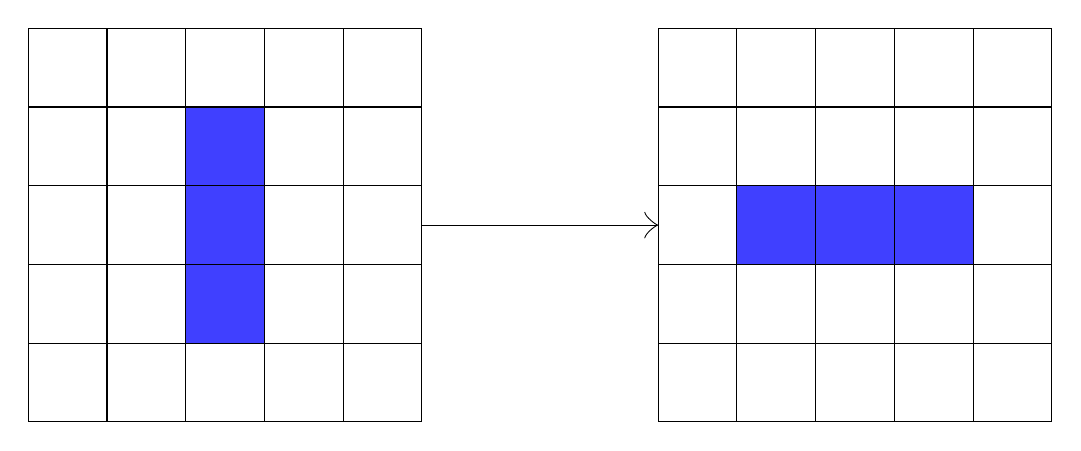
\begin{tikzpicture}
      \begin{scope}[xshift=-4cm]
        \grid{
          {0,0,0,0,0},
          {0,0,1,0,0},
          {0,0,1,0,0},
          {0,0,1,0,0},
          {0,0,0,0,0}}
        \node(arrstart) at (5,-2.5) {};
      \end{scope}
      \begin{scope}[xshift=4cm]
        \grid{
          {0,0,0,0,0},
          {0,0,0,0,0},
          {0,1,1,1,0},
          {0,0,0,0,0},
          {0,0,0,0,0}}
        \node(arrend) at (0,-2.5) {};
      \end{scope}
      \draw[-{Classical TikZ Rightarrow[length=5pt]}] (arrstart.center) -- (arrend.center);
    \end{tikzpicture}
    \subcaption{The pattern itself}
  \end{subfigure}\\
  \begin{subfigure}{\linewidth}
    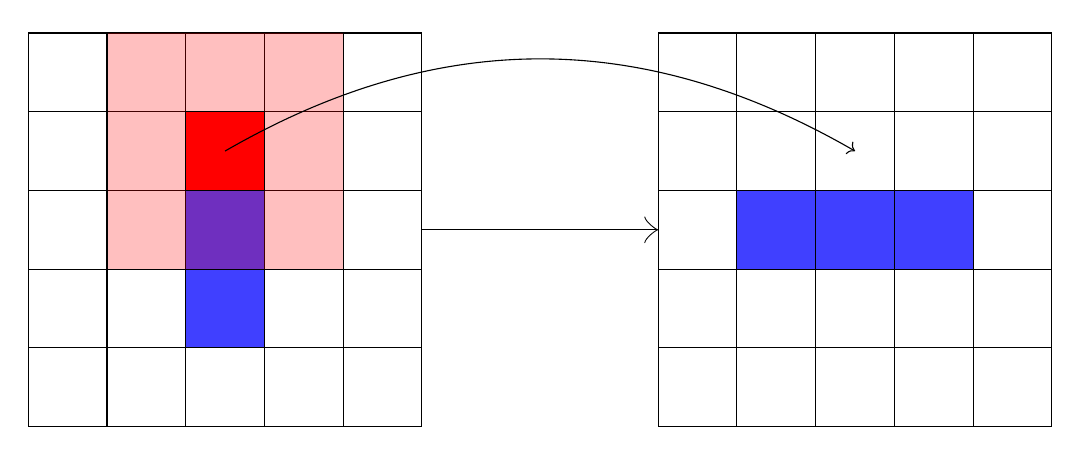
\begin{tikzpicture}
      \begin{scope}[xshift=-4cm]
        \grid{
          {0,0,0,0,0},
          {0,0,1,0,0},
          {0,0,1,0,0},
          {0,0,1,0,0},
          {0,0,0,0,0}}
        \node(arrstart) at (5,-2.5) {};
        \node(first) at (2.5,-1.5) {};
        \draw[fill=red,fill opacity=0.25] (1,0) rectangle ++(3,-3);
        \draw[fill=red] (2,-1) rectangle ++(1,-1);
      \end{scope}
      \begin{scope}[xshift=4cm]
        \grid{
          {0,0,0,0,0},
          {0,0,0,0,0},
          {0,1,1,1,0},
          {0,0,0,0,0},
          {0,0,0,0,0}}
        \node(arrend) at (0,-2.5) {};
        \node(second) at (2.5,-1.5) {};
      \end{scope}
      \draw[-{Classical TikZ Rightarrow[length=5pt]}] (arrstart.center) -- (arrend.center);
      \draw[->] (first.center) to[bend left] (second.center);
    \end{tikzpicture}
    \subcaption{With a live cell highlighted}
    \label{fig:GoLli}
  \end{subfigure}
  \begin{subfigure}{\linewidth}
    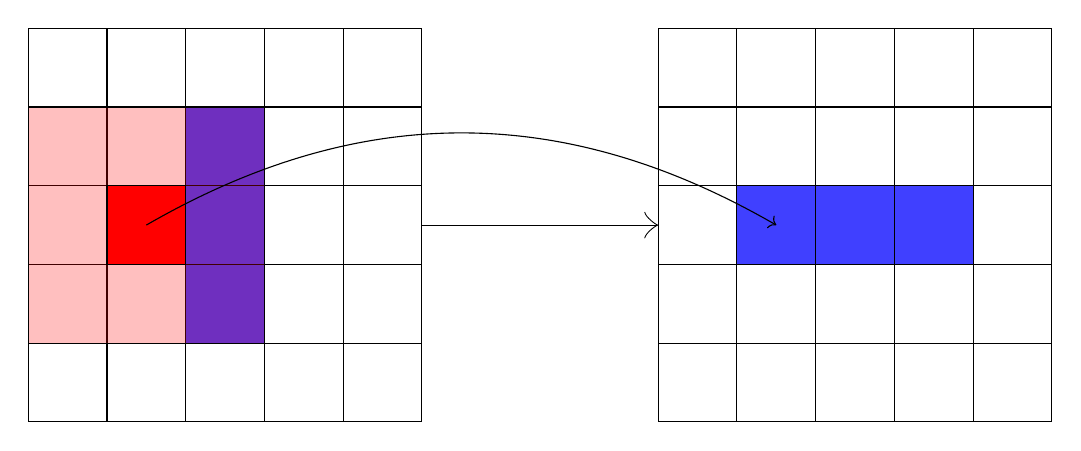
\begin{tikzpicture}
      \begin{scope}[xshift=-4cm]
        \grid{
          {0,0,0,0,0},
          {0,0,1,0,0},
          {0,0,1,0,0},
          {0,0,1,0,0},
          {0,0,0,0,0}}
        \node(arrstart) at (5,-2.5) {};
        \node(first) at (1.5,-2.5) {};
        \draw[fill=red,fill opacity=0.25] (0,-1) rectangle ++(3,-3);
        \draw[fill=red] (1,-2) rectangle ++(1,-1);
      \end{scope}
      \begin{scope}[xshift=4cm]
        \grid{
          {0,0,0,0,0},
          {0,0,0,0,0},
          {0,1,1,1,0},
          {0,0,0,0,0},
          {0,0,0,0,0}}
        \node(arrend) at (0,-2.5) {};
        \node(second) at (1.5,-2.5) {};
      \end{scope}
      \draw[-{Classical TikZ Rightarrow[length=5pt]}] (arrstart.center) -- (arrend.center);
      \draw[->] (first.center) to[bend left] (second.center);
    \end{tikzpicture}
    \subcaption{With a dead cell highlighted}
    \label{fig:GoLdi}
  \end{subfigure}
  \caption{Evolving a pattern by one generation using Conway's Game of Life}
  \label{fig:GoL}
\end{figure}

The effect of these rules can be seen in Figure~\ref{fig:GoL},
  which shows the effect of one application of the above rules on a small starting pattern.
Dead cells are drawn in white and live cells are drawn in blue.

To illustrate the rules more clearly, in Figure~\ref{fig:GoLli} one live cell is highlighted in red.
Its eight surrounding cells are highlighted in a lighter colour.
If we consider the middle cell, we can see that it is next to only one live cell,
  so by the Rule~\ref{itm:golao} above it turns into a dead cell.
Figure~\ref{fig:GoLdi} is similar, except that a dead cell is highlighted instead of a live cell.
This cell has three neighbouring live cells, so by Rule~\ref{itm:gold3} it becomes alive in the next generation.

\section{About Cabasa}
\label{sec:about}

Cabasa is an application for running \textbf{2D} cellular automata on (at the moment) a \textbf{finite} grid.
It aims to support any CA, unlike existing applications which can only support certain classes of CAs.
Do note that it does not aim to be particularly fast; if you want a very fast simulator, another application is probably better.

\chapter{Quickstart}
\label{chap:qstart}

To select a new rule, press the \menu{Control > Set Rule} menu item.
This opens a rule-selection dialog, where you can type a rule in or select a preexisting rule.
Cabasa comes with a set of predefined rules; to select one of these, use the menu item \menu{File > Open}.
In this example, we'll use the \texttt{life.alp} rule; it implements the \emph{Game of Life} rule described in Section~\ref{sec:whatisca}.
Selecting this rule and pressing the `Ok' button will make its contents appear in the dialog.
Press the \texttt{Set Rule} button to change the current rule to the rule which you have selected.

Now we can draw a pattern on the grid to use with this rule.
Select state \texttt{1} from the dropdown box at the top of the window marked `Current drawing state' (see screenshot, Figure~\ref{fig:mainwin}).
After this you should be able to draw patterns on the grid.
If you press the \keys{M} key, you can click and drag to move around; pressing \keys{D} gets you back to drawing mode.

To run the selected CA rule on your pattern, press the triangular `Play' button on the left of the screen;
  pressing it again should pause the evolution.
You should observe the pattern changing;
  this is due to the repeated application of the \emph{Game of Life} rules as described above.

\chapter{Getting Started}
\label{chap:gstart}

\section{User interface}
\label{sec:ui}

\begin{figure}[h]
  \centering
  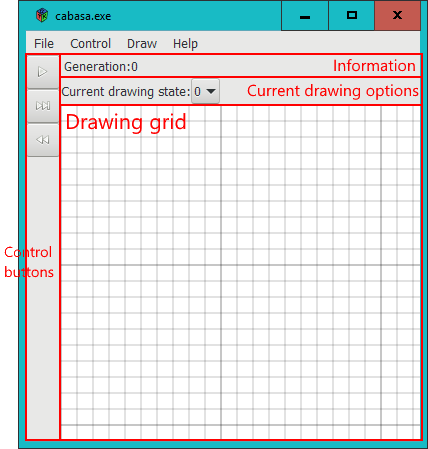
\includegraphics[scale=.8]{screenshot.png}
  \caption{Cabasa Main Window}
  \label{fig:mainwin}
\end{figure}

The main window, shown on Figure~\ref{fig:mainwin}, is composed of several parts.

The large grid in the middle shows the current state of the CA grid.
The user can draw on the grid, move around to show the rest of the grid, and use the currently loaded CA to evolve the pattern shown on the grid.

The information pane, just below the menu, shows various pieces of information about the current application state.
Currently it only shows the current generation,
  but it is expected that it will contain more information in future versions of Cabasa.

The drawing options pane, below the information pane, shows options related to drawing.
Again, there is currently only one thing shown here, but future versions may add more.
This pane will be disabled if drawing mode is not enabled.

\section{Drawing and Moving}
\label{sec:drming}

The application starts in \emph{drawing mode}.
In this mode, clicking and dragging on the grid changes the state of each cell the cursor passes over.

By default, the grid starts with all grid cells set to state 0 and the \emph{drawing state} also set to 0,
  so nothing happens when you try to draw on the grid.
However, by changing the selected state (next to the text `Current drawing state'), other states can be chosen.
For instance, if state 1 is selected, then clicking and dragging on the grid will change the cells under the cursor to state 1.
Note that the states are numbered starting from 0, not 1,
  so to select e.g.\ the second state you have declared you need to select state 1, not state 2.

Moving around the grid requires another mode, \emph{move mode}.
This mode can be selected from the \menu{Draw > Mode} menu, or by pressing the \keys{M} key.
You can get back to drawing mode by using the \menu{Draw} menu, or by pressing the \keys{D} key.
In this mode, clicking and dragging will not draw on the grid, but rather will move or pan around the grid.
Enabling this mode will also disable the `drawing options' pane.

In any mode, you can also zoom in and out using the mouse wheel.
At the moment, zooming always works relative to the top-leftmost point.
This means that if you have a pattern drawn in the middle of the grid and it suddenly vanishes when you zoom in,
  try moving to the bottom left to try find it again.

If you zoom out far enough, you will notice that the grid abruptly comes to an end at a certain point.
This is because the grid is finite.
However, the grid `wraps around' at its edges; that is, if you move off one edge of the paper, you reappear at the opposite edge.
For instance, the cell immediately above the topmost cell is considered to be the bottommost cell.

\section{Changing the Rule}
\label{sec:chngrule}

The current CA can be changed using the \menu{Control > Set Rule} menu item.
This opens a window where you can type in a specification of a CA rule.

Two specification languages are supported: \emph{ALPACA} and \emph{Haskell}.
You can switch between these using the option box at the bottom of the window.
For more details on these formats, see Chapter~\ref{chap:speccas}.

To accept a specification, press the `Set Rule' button at the bottom of the window.
This will interpret the specification and load it into the main window.
If the specification is invalid, it will show an error dialog instead.

After the rule is set, you will be able to draw patterns in this rule on the grid in the main window.
The set of states available for drawing through the `current drawing state' option will change to reflect the new rule.
Since the set of allowed states could have changed, the grid will be cleared after each rule change.

For more details on how to specify a CA, see Chapter~\ref{chap:speccas},
  but if you want to play around with a specification now then you can copy the following Game of Life specification into the `Set Rule' window:

\begin{verbatim}
state Dead  " "
  to Alive when 3 Alive and 5 Dead;
state Alive "*"
  to Dead when 4 Alive or 7 Dead.
\end{verbatim}

This is written in ALPACA, so make sure that the ALPACA language is selected before setting the rule.

\section{Running CAs}
\label{sec:running}

A set of \emph{control buttons} can be seen on the left of the window.
These buttons are used to actually run the CA once a rule has been loaded and a pattern has been drawn.

To run one generation of the CA, use the middle button.
This operation is called \emph{stepping}.
You can repeatedly press this button to run the rules more than once.

The topmost button will repeatedly step the CA.
This operation is generally referred to as \emph{running} the CA.
Currently the rate at which the rules are applied cannot be changed;
  this will be corrected in future versions.
After this button has been pressed, the icon will change to a pause icon.
As this suggests, the button can be pressed again to pause the CA.
Pressing it again will allow the CA to be run again.

To reset the CA after you have run or stepped it, use the bottom `reset' button.
This button will restore the original state of the CA after you have pressed the `step' or `run' buttons.
If you haven't run the CA, then it doesn't do anything.

To clear the pattern, use the \menu{Draw > Clear} menu item.
This resets the generation, clears the pattern and moves the grid so that the top-left corner is displayed
  (as in the start of the program).

\section{Opening and Saving}
\label{sec:opsav}

Cabasa has the ability to open and save both rules and patterns.
This can be done through the \menu{File > Open} and \menu{File > Save As} menu items on the CA specification window and main window respectively.
\textit{Save} (as opposed to \textit{save as}) functionality has not yet been implemented, but will be implemented in a later version of Cabasa.

In more detail:

\begin{itemize}
\item To \textbf{save the current rule}, use the \menu{Control > Set Rule} menu item on the main window to open the CA selection window.
  Then press the \menu{File > Save As} menu item on the CA selection window to show a file selection dialog where you can save the current rule.
  Ensure that the correct format (ALPACA or Haskell) is selected before saving.
\item To \textbf{open a previously saved rule}, use the \menu{Control > Set Rule} menu item on the main window to open the CA selection window.
  Then press the \menu{File > Open} menu item on the CA selection window to show a file selection dialog where you can open a previously saved rule.
  If your rule is not listed, try changing the file format (ALPACA or Haskell) at the bottom of the window.
  After the rule has been opened, press the \textit{Set Rule} button at the bottom of the window to load it as the current rule.
\item To \textbf{save the current pattern}, use the \menu{File > Save As} menu item on the main window to show a file selection dialog where you can save the current pattern.
\item To \textbf{open a previously saved pattern}, use the \menu{File > Open} menu item on the main window to show a file selection dialog where you can open a previously saved pattern.
  If the pattern has been saved with a different rule to the rule currently active,
    a dialog box will be shown asking you if you want to switch rules.
\end{itemize}

\subsection{The Local Rules and Patterns Directories}
\label{sec:locdirs}

By default, Cabasa maintains two directories, called \texttt{Patterns} and \texttt{Rules}.
As the names suggest, these are the default directories for saved patterns and rules respectively.
Although there is nothing special about these directories in and of themselves --- you can save patterns and rules anywhere ---
  the \texttt{Rules} directory is the place where Cabasa looks for unknown rules,
  so you need to save your rules there if you want them to be found automatically when you open a pattern.

\chapter{Specifying CAs}
\label{chap:speccas}

\section{Languages}
\label{sec:speclangs}

Cabasa supports two languages to specify CAs: \emph{ALPACA} and \emph{Haskell}.

ALPACA is a language created by Chris Pressey specifically for the specification of CAs.
Cabasa currently supports ALPACA version 1.1.

Cabasa also allows CAs to be implemented in the Haskell programming language.
As Haskell is a full-featured programming language, this approach is more powerful than using ALPACA,
  but is extremely difficult if you do not already know Haskell.

\section{Using ALPACA}
\label{sec:usalp}

The reference manual for ALPACA version 1.1 is a very good guide for learning about the various features of ALPACA.
It is available at the following web address: \url{https://github.com/catseye/ALPACA/blob/0b2d57b8739dc240969c62c8e1cd13c1863770e0/doc/ALPACA.markdown}.
Cabasa should support all the features outlined in that manual
  \textbf{except} for the initial configuration, which is currently ignored.

Do note however that for technical reasons\footnotemark,
  the `examples' in the ALPACA manual are actually written in a format called `Falderal' and not plain ALPACA;
  the ALPACA translation can be found by reading the parts of the example which are after the \texttt{|} characters.
For instance, take this example from the manual:

\begin{verbatim}
| state Space " ";
| state Up "U"
|   to ^ when true;
| state Down "D"
|   to v when true
| begin
| DDD
| UUU
= -----
= UUU
= DDD
= -----
\end{verbatim}

For this example, the ALPACA which you would actually type is the following portion:

\begin{verbatim}
state Space " ";
state Up "U"
  to ^ when true;
state Down "D"
  to v when true
begin
DDD
UUU
\end{verbatim}

\footnotetext{In more detail: the `examples' are actually runnable tests containing an embedded description of the expected output as well.}

\section{Using ALPACA Stylesheets}
\label{sec:stys}

The \emph{ALPACA Stylesheets} format is a simple way to change the styling of a CA specified using ALPACA.
The format is documented at \url{https://github.com/catseye/ALPACA/blob/0b2d57b8739dc240969c62c8e1cd13c1863770e0/doc/ALPACA.markdown#alpaca-stylesheets-10}.

To open the ALPACA Stylesheets window, use the \menu{Draw > Edit Stylesheet} menu item.
This opens a window where you can edit the current stylesheet using the textbox in the middle of the screen,
  and then set it using the `Set Stylesheet' button at the bottom.
You can also use the \menu{File > Open} and \menu{File > Save As} menu items to open and save stylesheets respectively.

\section{Using Haskell}
\label{sec:ushs}

\textbf{Note:} If you don't know Haskell then feel free to skip this section.

\vspace{2ex}

\noindent It is also possible to use the Haskell programming language to specify CAs.
This functionality relies on a library created specifically for Cabasa.
Its documentation can be found \href{haskell/index.html}{here}.

A Haskell CA specification consists of a module containing a value \texttt{myCA ::\ \href{haskell/Hint-Interop.html\#t:CAVals}{CAVals}}.
You should also import the \hreftt{haskell/CA.html}{CA} and \hreftt{haskell/Hint-Interop.html}{Hint.Interop} modules,
  as types and values from these modules are used to define a CA.
With the exception of these provisos, a CA specification is a completely normal Haskell module,
  meaning that you can enable GHC extensions (e.g. \texttt{-XRecordWildCards} is particularly useful),
  import other modules (as long as they are in \texttt{base})
  and generally do anything you could normally do in a Haskell module.

The \texttt{myCA ::\ \href{haskell/Hint-Interop.html\#t:CAVals}{CAVals}} value (mentioned above) is the central part of the CA definition.
This value is an existentially quantified wrapper around a \hreftt{haskell/Hint-Interop.html\#t:CAVals-39-}{CAVals\textquotesingle} record,
  which encapsulates the various pieces of information needed for Cabasa to use the CA.
The details of these fields can be found in the documentation.

An annotated example of a CA definition (in this case, Conway's Game of Life) can be found in Listing~\ref{lst:agol}.
This is adapted from the example \href{haskell/CA.html}{here}.
However, this rule would usually be written as Listing~\ref{lst:ugol},
  which uses the utility functions from \href{haskell/CA-Utils.html}{\texttt{CA.Utils}}.

\begin{listing}
\begin{minted}{haskell}
{-# LANGUAGE LambdaCase      #-}
{-# LANGUAGE RecordWildCards #-}

module Life where

import CA
import Hint.Interop

data State = Alive | Dead

myCA :: CAVals
myCA = CAVals $ CAVals' {..}
  where
    -- This is the rule itself. It needs to return a Rand though, so the result
    -- is fed to `pure'.
    _rule = pure . conwayLife

    -- This is the list of states which are shown in the state selection box;
    -- `Dead' is shown as state 0 and `Alive' is shown as state 1.
    _states = [Dead, Alive]

    -- This is the pattern shown when the rule is first loaded.
    _defaultPattern = fromList $ replicate 100 $ replicate 100 Dead

    -- This is the function which determines what colour each state is displayed
    -- as.
    _state2color Dead  = (0,0,0)
    _state2color Alive = (1,1,1)

    -- These two functions convert states to integers and vice versa. They are
    -- used to save and load patterns to and from a file.
    _encodeInt Dead  = 0
    _encodeInt Alive = 1
    _decodeInt 1 = Alive
    _decodeInt _ = Dead

conwayLife :: Universe State -> State
conwayLife u = case extract u of
    Dead ->
        if count (experiment mkNbhd u) == 3
        then Alive
        else Dead
    Alive ->
        if count (experiment mkNbhd u) `elem` [2, 3]
        then Alive
        else Dead
  where
    mkNbhd (Point x y) = [ Point (x-1) (y-1)
                         , Point  x    (y-1)
                         , Point (x+1) (y-1)
                         , Point (x-1)  y
                         , Point (x+1)  y
                         , Point (x-1) (y+1)
                         , Point  x    (y+1)
                         , Point (x+1) (y+1)
                         ]

 count = sum . fmap (\case { Alive -> 1 ; Dead -> 0 })
\end{minted}
\caption{Annotated Conway's Game of Life in Haskell}
\label{lst:agol}
\end{listing}

\begin{listing}[!b]
\begin{minted}{haskell}
{-# LANGUAGE RecordWildCards #-}

module Life where

import CA
import Hint.Interop

data State = Alive | Dead deriving (Eq)

myCA :: CAVals
myCA = CAVals $ CAVals' {..}
  where
    _rule = pure . conwayLife
    _states = [Dead, Alive]
    _defaultPattern = fromList $ replicate 100 $ replicate 100 Dead
    _state2color Dead  = (1,1,1)
    _state2color Alive = (0,0,0)
    _encodeInt Dead  = 0
    _encodeInt Alive = 1
    _decodeInt 1 = Alive
    _decodeInt _ = Dead

conwayLife :: Universe State -> State
conwayLife u =
    let aliveCount = count (==Alive) $ experiment (moore False) u in
        case extract u of
            Dead ->  if aliveCount == 3          then Alive else Dead
            Alive -> if aliveCount `elem` [2, 3] then Alive else Dead
\end{minted}
\caption{Conway's Game of Life in Haskell using \hreftt{haskell/CA-Utils.html}{CA.Utils}}
\label{lst:ugol}
\end{listing}

\appendix

\chapter{Sample Patterns and Rules}
\label{chap:samps}

Cabasa comes with a set of predefined example patterns and rules.
These are located in the default pattern and rule directories,
  so to access them you can simply use the relevant \menu{File > Open} menu items.

The predefined rules are:

\begin{description}
\item[life.alp] An ALPACA implementation of Conway's Game of Life
\item[bbrain.alp] An ALPACA implementation of \emph{Brian's Brain}, another well-known CA.
  This CA tends to explode chaotically, creating fascinating dynamic patterns.
\item[wireworld.alp] An ALPACA implementation of \emph{Wireworld}, a CA designed to simulate computer circuits.
  For more information on WireWorld, see \url{https://www.quinapalus.com/wires0.html}
\item[life.hs] A Haskell implementation of Conway's Game of Life.
  This in particular is a good template to start coding a CA in Haskell.
\item[langton.hs] A Haskell implementation of \textit{Langton's Ant}, a well-known CA simulating a moving `ant'.
  For more information on Langton's Ant, see \url{https://en.wikipedia.org/wiki/Langton%27s_ant}
\end{description}

The predefined patterns are:

\begin{description}
\item[pi.mcl \textnormal{and} r.mcl] The \emph{pi-heptomino} and \emph{r-pentomino}, two patterns which evolve in an interesting way when run using Conway's Game of Life.
\item[gates.mcl] The \textsc{and} and \textsc{or} logic gates in Wireworld.
\item[langton.mcl] An initial configuration for Langton's Ant.
\end{description}

\end{document}

% Local Variables:
% TeX-command-extra-options: "-shell-escape"
% End:
